\begin{figure*}
  \centering
  \begin{subfigure}[b]{\textwidth}
    \centerline{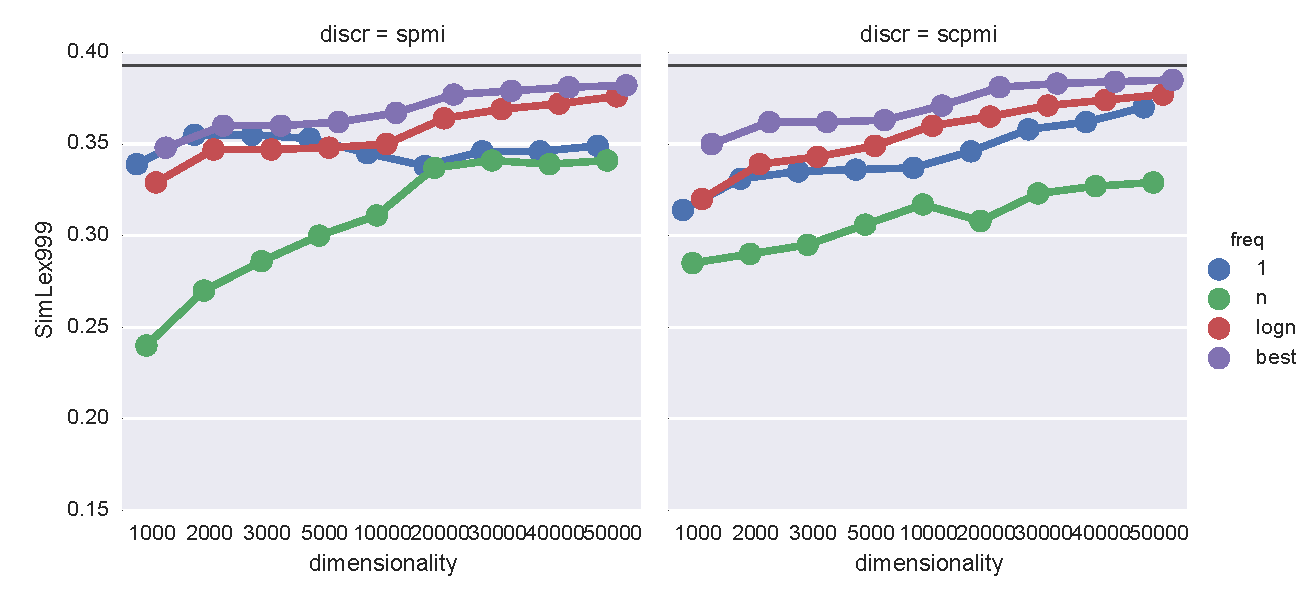
\includegraphics[width=1.1\textwidth]{supplement/figures/SimLex999-best}}
    \caption{\textbf{SimLex-999.} The black line refers to the score of 0.393.
      This work: 0.385,
      SGNS: 0.438,
      GloVe: 0.398.
    }
    \label{fig:simlex-ppmi-best-simlex}
  \end{subfigure}

  \begin{subfigure}[b]{\textwidth}
    \centerline{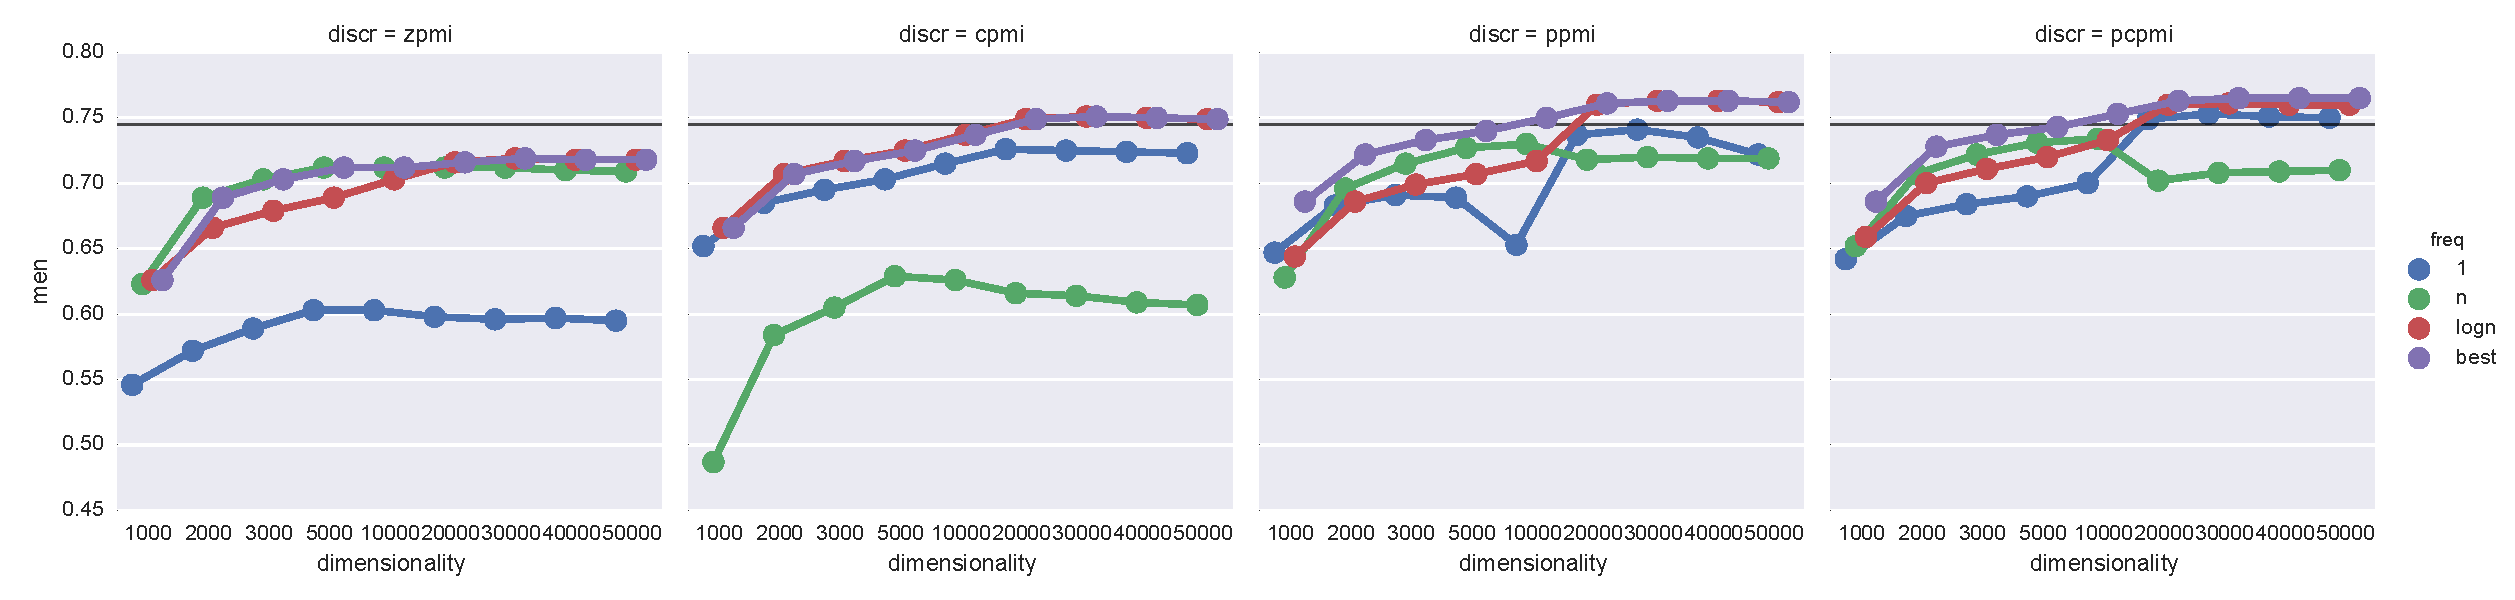
\includegraphics[width=1.1\textwidth]{supplement/figures/men-best}}
    \caption{\textbf{MEN.} The black line refers to the score of 0.745.
      This work: 0.765,
      SGNS: 0.774,
      GloVe: 0.729.
    }
    \label{fig:simlex-ppmi-best-men}
  \end{subfigure}

  \caption{\textbf{SPMI best configurations.} Black line shows the best count models reported by \protect\newcite{TACL570}. We also give our best score, SGNS and GloVe numbers from that study for comparison.}
  \label{fig:simlex-ppmi-best}
\end{figure*}

%%% Local Variables:
%%% mode: latex
%%% TeX-master: "paper"
%%% End:
